%% %%%%%%%%%%%%%%%%%%%%%%%%%%%%%%%%%%%%%%%%%%%%%%%%%%% %%
%%        TCC de Rafael M. Lins de Araújo, 2016        %%
%% %%%%%%%%%%%%%%%%%%%%%%%%%%%%%%%%%%%%%%%%%%%%%%%%%%% %%

%% Preâmbulo (configurações, pacotes e tudo mais)
%% Preambulo LaTeX: Define classes e características do documento
%% Definição do docuemnto
\documentclass[
	%article,			% Define que este será um artigo (e não uma tese/monografia/relatório)
	12pt,				% Fonte: 12pt
	oneside,			% Impressão: oneside = 1 face, twoside = 2 faces (frente-e-verso)
    %openright,			% capítulos começam em página ímpar (use apenas se usar "twoside")
	a4paper,			% Tamanho do Papel: A4
    chapter=TITLE,		% Todos os capítulos devem ficam em caixa alta
    section=TITLE,		% Todas as seções devem ficar em caixa alta
	english,			% Adiciona Idioma para Hifenização: Inglês
    %spanish,			% Adiciona Idioma para Hifenização: Espanhol
    %french,			% Adiciona Idioma para Hifenização: Francês
	brazil				% Adiciona Idioma para Hifenização: Português do Brasil (o último idioma se torna o principal do documento)
]{abntex2}				% Utilizar ABNTeX2



%% Tipografia
%% Abra este arquivo e selecione uma das opções de fonte nele. A padrão é Times.
%% Tipografia / Fontes
%% AVISO: Todas essas fontes são *bastante semelhantes* aos nomes com as quais as descrevo. Entenda: são iguais, só que oficialmente com outro nome.

%% %%%%%%%%%%%%%%%%%%%%%%%%%%%%%%%%%%%%%%%%%%%%%%%%%%%%% %%
%% Comente todas as outras fontes que você não vai usar! %%
%% %%%%%%%%%%%%%%%%%%%%%%%%%%%%%%%%%%%%%%%%%%%%%%%%%%%%% %%

%% Latin Modern (fonte padrão do LaTeX, Computer Modern, mas com suporte a caracteres acentuados)
%% Considerada a mais clássica e bonita
%\usepackage{lmodern}



%% Times
%% Considerada a mais confortável de ler quando impresso
\usepackage{mathptmx}

%% Variação da mesma fonte, com minúsculas diferenças entre uma e outra (coisas bastante técnicas como kerning, aliasing e afins) - Essa tem revisões frequentes
%\usepackage{newtxtext} \usepackage{newtxmath}



%% Arial
%% Considerada mais confortável de ler num computador
%% ** Oficialmente recomendada pelo manual de formatação do IFPI **
%\usepackage{helvet} \renewcommand{\familydefault}{\sfdefault}



%% Palatino
%% Uma opção mais elegante à Times
%\usepackage{newpxtext}



%% Kepler
%% Variação evoluída da Palatino, com várias pequenas diferenças e refinamentos
%\usepackage{kpfonts}



%% Libertine
%% Uma fonte estilo Serif comum no Linux
%\usepackage{libertine} %\usepackage[libertine]{newtxmath}



%% Pacotes usados pelo documento (se não entender não mexa, hehehe)
\usepackage{courier}                    % Permite a utilização da fonte Courier (para códigos-fonte)
\usepackage[T1]{fontenc}				% Seleção de códigos de fonte.
\usepackage[utf8]{inputenc}				% Codificação do documento (conversão automática dos acentos)
\usepackage{indentfirst}				% Indenta o primeiro parágrafo de cada seção.
\usepackage{nomencl} 					% Usado pela Lista de símbolos
\usepackage{color}						% Controle das cores
\usepackage{graphicx}					% Inclusão de gráficos
\usepackage{float}						% Melhorias para posicionamento de gráficos e tabelas
\usepackage{microtype} 					% Melhorias na justificação
\usepackage{lastpage}   		        % Dá acesso ao número da última página do documento
\usepackage{booktabs}					% Comandos para tabelas
\usepackage{multirow, array}			% Múltiplas linhas e colunas em tabelas
\usepackage[hyphenbreaks]{breakurl}		% Hifenação para URLs no texto
\usepackage[table,xcdraw]{xcolor}       % Cores para algumas tabelas especiais
\usepackage[brazilian,hyperpageref]{backref}	 % Inclui nas Referências as páginas onde há as citações
\usepackage{simplecd}                   % Pacote para gerar capa do CD
\usepackage[final]{pdfpages}            % Pacote para incluir um PDF dentro de outro (ficha catalográfica)



%% Adiciona as alterações do ABNTeX-IFPI
\usepackage{abntex-ifpi/abntex-ifpi}	% Modificações do ABNTeX para o IFPI
\usepackage{abntex-ifpi/tikz-uml}	    % Pacote Tikz UML para criar UML no LaTeX



%% Metadados
%% Configurações dos metadados do PDF
\makeatletter
\hypersetup{
  pdftitle={\@title}, 
  pdfauthor={\@author},
  pdfsubject={\@title},
  pdfcreator={LaTeX, abnTeX2, {abnTeX\-ifpi}},
  %% Coloque aqui suas palavras-chave, cada uma entre chaves: {palavra}{palavra}{outra palavra}...
  pdfkeywords={financiamento coletivo}{empreendimento social}{crowdfunding}{impacto social}{social impact}{social entrepreneurship},
  colorlinks=true,			% Visual dos Links: false = caixas; true = colorido
  linkcolor=cor-link,		% Cor dos Links Internos (preto)
  citecolor=cor-link,		% Cor de Links para Bibliografia (preto)
  filecolor=cor-link,		% Cor para Links a Arquivos (preto)
  urlcolor=cor-link,		% Cor para Links a URLs (preto)
  bookmarksdepth=4
}
\makeatother



%% Metadados
%% %%%%%%%%%%%%%%%%%%%%%%%%%%%%%%%%%%%%%%%%%%%%%%%% %%
%% Metadados do trabalho
%% AVISO: Todos esses dados serão automaticamente convertidos para caixa alta onde necessário
%% %%%%%%%%%%%%%%%%%%%%%%%%%%%%%%%%%%%%%%%%%%%%%%%% %%

%% Título
\titulo{Ajuda.Ai - Uma solução em Software para Crowdfunding Social}

%% Autor
\autor{Rafael Madureira Lins de Araújo}

%% Nome do Curso (usado para a Capa do CD)
\nomedocurso{Análise e Desenvolvimento de Sistemas}

%% Local de publicação
\local{Teresina, Piauí}

%% Preâmbulo do trabalho
\preambulo{Projeto apresentado à Banca Examinadora como requisito para aprovação na disciplina de Trabalho de Conclusão de Curso II do Curso Superior de Tecnologia em Análise e Desenvolvimento de Sistemas do Instituto Federal de Educação, Ciência e Tecnologia do Piauí.}

%% Orientador
%% "M\textsuperscript{e}." = Abreviação oficial para "Mestre"
\orientador{Prof. M\textsuperscript{e}. Ely da Silva Miranda}

%% Tipo de Trabalho
%% - Monografia
%% - Tese (Mestrado)
%% - Tese (Doutorado)
%% - Relatório técnico
\tipotrabalho{Monografia}

%% Data do Trabalho
\data{2017}

%% Nome da Instituição (para a capa)
\instituicao{INSTITUTO FEDERAL DE EDUCAÇÃO, CIÊNCIA E TECNOLOGIA DO PIAUÍ
\\
CAMPUS TERESINA CENTRAL
\\
TECNOLOGIA EM ANÁLISE E DESENVOLVIMENTO DE SISTEMAS}

%% Primeiro membro da banca examinadora
\membroum{Prof. M\textsuperscript{e}. Rogério da Silva}

%% Segundo membro da banca examinadora
\membrodois{Prof. M\textsuperscript{e}. Duany Dreyton Bezerra Sousa}

%% Terceiro membro da banca examinadora
%\membrotres{Prof. Dr. Ney Paranaguá de Carvalho}

%% Data da apresentação do trabalho
%% Se não souber a data da apresentação, utilize \underline{\hspace{3.5cm}}
%% Isso cria um sublinhado de 3.5cm, onde você pode escrever a data depois!
%\dataapresentacao{04 de Abril de 2017}
\dataapresentacao{\underline{\hspace{3.5cm}}}



%% Configuração do "Citado nas páginas"
%% Configuração das Citações

%% Estilo
\usepackage[num]{abntex2cite}			% Citações numéricas
%\usepackage[alf]{abntex2cite}			% Citações "AUTOR, ano"

%% Colocar entre parênteses ou colchetes?
%% Padrão: Parênteses
%% * Fica mais agradável usar colchetes quando se usa citações numéricas
\citebrackets[]							% Comente essa linha e o documento usará parênteses


%% Configura o "Citado nas Páginas ..." nas referências
%% Não mexa nesse:
\renewcommand{\backref}{}

%% Esse é o texto do "Citado nas páginas ..."
\renewcommand*{\backrefalt}[4]{
	\ifcase #1
		Nenhuma citação no texto.
	\or
		Citado na página #2.
	\else
		Citado #1 vezes nas páginas #2.
	\fi}



%% Cores
%% Cores do Documento

%% Cor dos Links do PDF
%% Usando preto você "esconde" os links
\definecolor{cor-link}{RGB}{0,0,0}

%% Usando azul os links ficam visíveis (ruim para impressão)
%\definecolor{cor-link}{RGB}{8,40,75}



%% Cor para os quadros
%% Dê preferência a cores escuras.
%% Boa referência para cores: https://material.io/guidelines/style/color.html#color-color-palette
\definecolor{cor-quadro}{RGB}{5,28,63}		% Azul Escuro




%% Espaçamentos
%% Espaçamentos
%% O tamanho do parágrafo é dado por:
\setlength{\parindent}{1.3cm}

%% Espaçamento entre um parágrafo e outro:
%% O abntex diz: "tente também \onelineskip"
\setlength{\parskip}{0.2cm}

%% Início do Documento
\begin{document}

%% Documento será escrito em Português do Brasil
\selectlanguage{brazil}

%% Elementos pré-textuais: capa, folha de rosto, dedicatória, listas, sumário, etc.
%% %%%%%%%%%%%%%%%%%%%%%%%%%%%%%%%%%%%%%%%%% %%
%% Elementos Pré Textuais
%% ----------------------
%% 
%% Segundo o manual do IFPI, eles devem ser os seguintes (nessa ordem):
%%  1. Capa (obrigatório)
%%  2. Folha de rosto (obrigatório)
%%  3. Errata (opcional)
%%  4. Folha de aprovação (obrigatório)
%%  5. Dedicatória (opcional)
%%  6. Agradecimentos (opcional)
%%  7. Epígrafe (opcional)
%%  8. Resumo (obrigatório)
%%  9. Abstract/Resumo em outra língua (obrigatório)
%% 10. Lista de Ilustrações (opcional)
%% 11. Lista de Tabelas (opcional)
%% 12. Lista de Abreviaturas e Siglas (opcional)
%% 13. Lista de Símbolos (opcional)
%% 14. Sumário (obrigatório)
%% %%%%%%%%%%%%%%%%%%%%%%%%%%%%%%%%%%%%%%%%% %%

%% 01: Capa
\imprimircapa



%% 02: Folha de Rosto
%% OBS: O asterisco indica que haverá ficha bibliográfica (só funciona para impressão frente-e-verso)
\imprimirfolhaderosto*



%% Ficha Catalográfica (acho que é melhor adicionar via \includepdf depois)
%% Se for incluir um outro PDF neste documento: 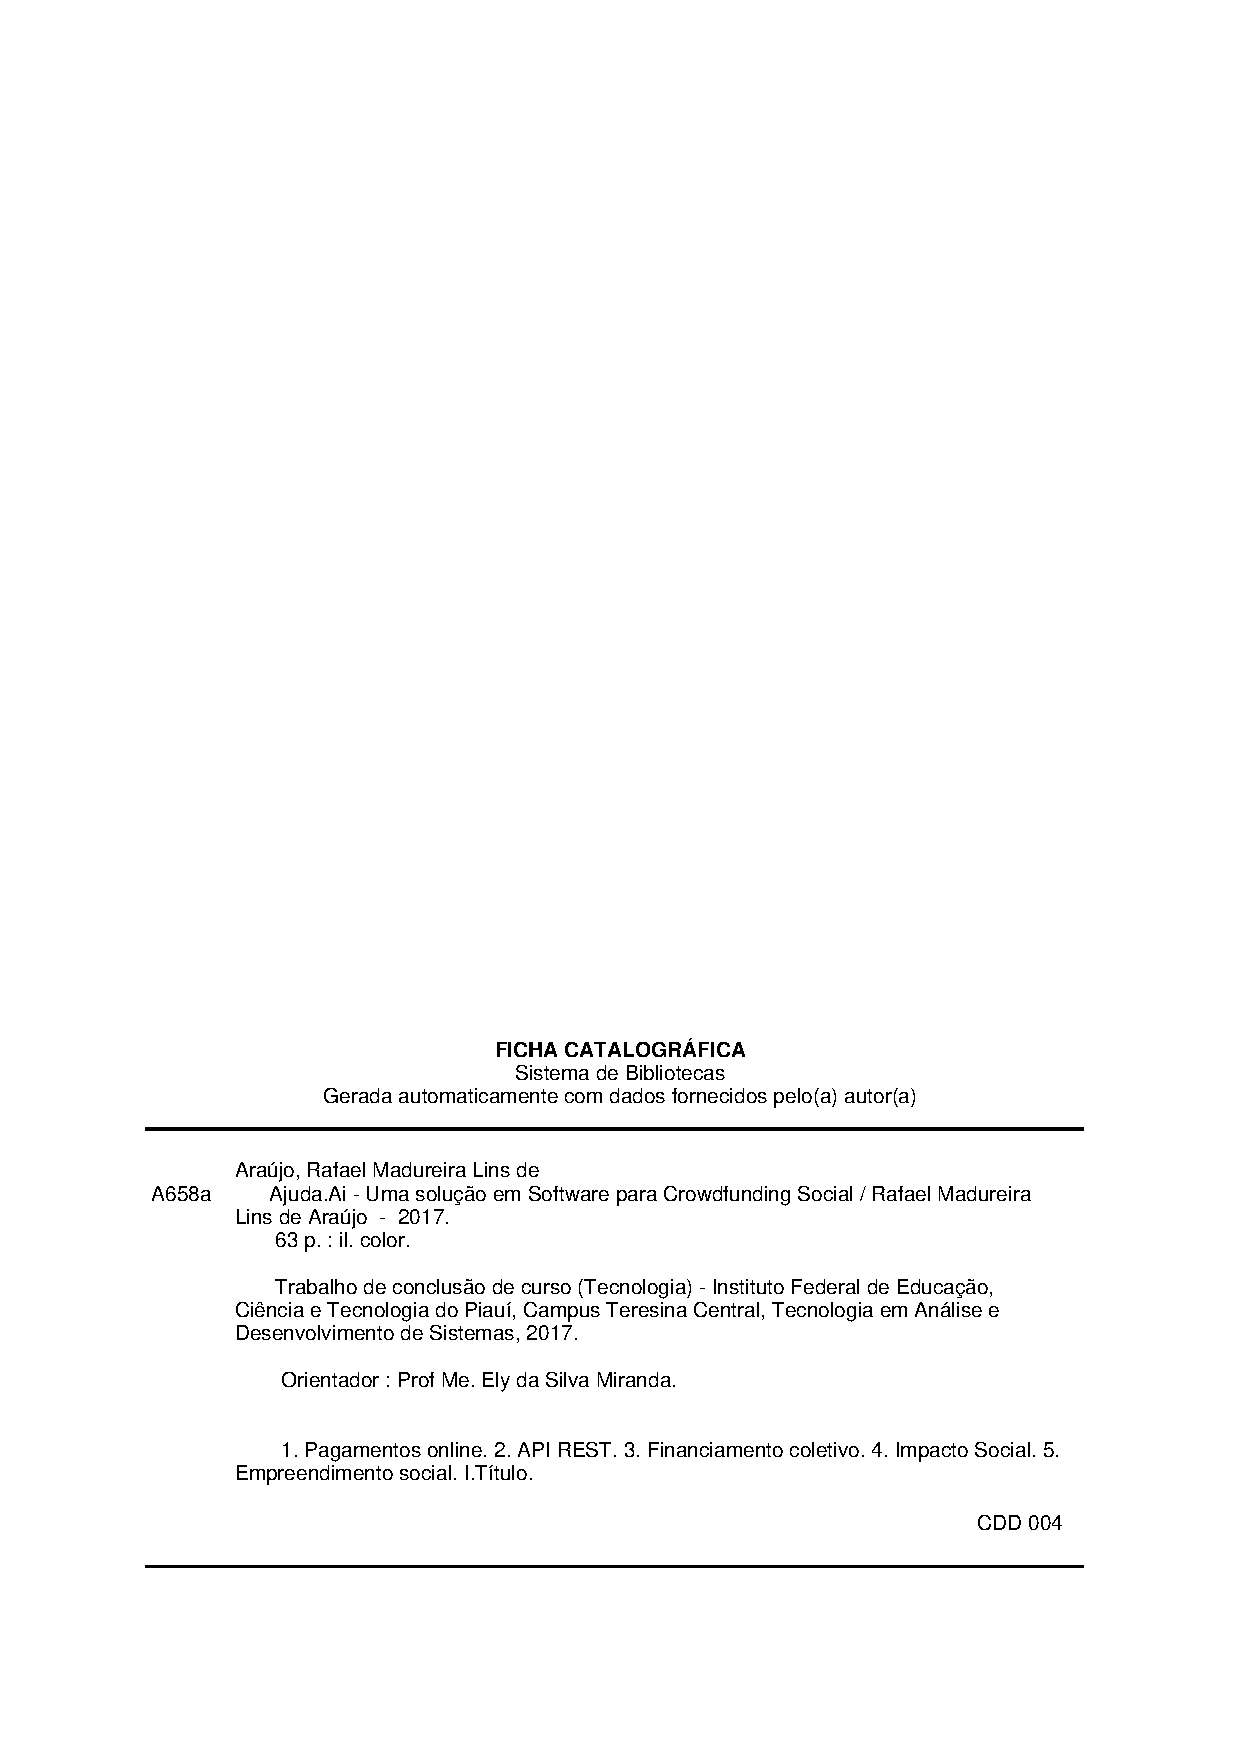
\includepdf{pasta-onde-está-a-ficha/ficha-catalografica.pdf}


%% 03: Errata
%% Errata
%\begin{errata}
%Elemento opcional da norma ABNT NBR14724 de 2011. Exemplo:
%
%\vspace{\onelineskip}
%
%FERRIGNO, C. R. A. \textbf{Tratamento de neoplasias ósseas apendiculares com reimplantação de enxerto ósseo autólogo autoclavado associado ao plasma rico em plaquetas}: estudo crítico na cirurgia de preservação de membro em cães. 2011. 128 f. Tese (Livre-Docência) - Faculdade de Medicina Veterinária e Zootecnia, Universidade de São Paulo, São Paulo, 2011.

%% Tabela de exemplo com os erros
%\begin{table}[htb]
%\center
%\footnotesize
%\begin{tabular}{|p{1.4cm}|p{1cm}|p{3cm}|p{3cm}|}
%  \hline
%   \textbf{Folha} & \textbf{Linha}  & \textbf{Onde se lê}  & \textbf{Leia-se}  \\
%    \hline
%    1 & 10 & auto-conclavo & autoconclavo\\
%   \hline
%\end{tabular}
%\end{table}
%
%\end{errata}



%% 04: Folha de Aprovação
\imprimirfolhadeaprovacao
%% Use esta se forem 4 membros na banca:
%\imprimirfolhadeaprovacaoduascolunas



%% 05: Dedicatória
%% Dedicatória do seu trabalho
\begin{dedicatoria}
	%% Empura o texto a seguir para a parte de baixo da página
	\vspace*{\fill}
    
    %% Alinhado a Direita
    \center
    \begin{flushright}
    	Dedico este trabalho a todos que acreditaram que ele sairia.
    \end{flushright}
    
    %% Descomente a linha seguir para deixar o texto centralizado verticalmente na página
    %% Lembre de comentar o "\begin{}" e "\end{}" acima para centralizar o texto da dedicatória.
	%\vspace*{\fill}
\end{dedicatoria}



%% 06: Agradecimentos
%% Agradecimentos
\begin{agradecimentos}
	Agradeço primeiramente a meus pais, família e Alaydes Morais que, assim como muitos, aguardaram pacientes pela conclusão do curso e me deram o apoio necessário para terminar a jornada.
    
    Agradeço aos amigos, virtuais e reais, pelas risadas, apoio, dicas e vários ``eu fiz meu TCC em \(N\) dias'' --- Em especial Rafael Soares, Rafarpo, Ebbitt, Rosenrot, Zenlee, Tajaro e Velinde.
    
    Agradeço profundamente aos mestres e professores que partilharam de seus conhecimentos por todos esses anos.
    
    Finalmente agradeço a meu orientador, Ely Miranda, por sua amizade, conselhos e excelentes revisões que tornaram esse trabalho possível.
\end{agradecimentos}



%% 07: Epígrafe
%% Epígrafe
%% Uma frase que lhe inspira ou a qual lhe inspirou a fazer este trabalho
\begin{epigrafe}
\vspace*{\fill}
\begin{flushright}
\emph{``Acredito que o poder de qualquer recurso - especialmente o financeiro - é potencializado quando vem com suporte da comunidade. O capital deixa de ser apenas capital, não mais apenas um meio para um fim. É uma coisa fundamentalmente diferente: uma expressão das melhores intenções de uma comunidade, suas esperanças para o futuro, seu desejo de participar em tornar esse futuro uma realidade. É uma asserção da sua confiança que quem receberá o capital vai liderar o caminho.'' \\ (Jessica Jackley, tradução livre)}
\end{flushright}
\end{epigrafe}



%% 08: Resumo
%% Resumo
\begin{resumo}
Empreendimentos sociais no Brasil historicamente têm bastante dificuldade em buscar o financiamento necessário para exercer de forma plena as atividades que necessitam e frequentemente se utilizam de campanhas de trabalho voluntário e doações de alimentos ou objetos usados. Apesar da redução de custos que trabalho voluntário e doações trazem é inegável a necessidade de dinheiro para custos como eletricidade, água e medicamentos. Campanhas de arrecadação financeira de organizações menores são comumente discretas, como pedir o troco de uma compra como uma pequena doação.

Para resolver esses problemas há soluções como buscar investidores, micro crédito junto a bancos comunitários, campanhas em mídias por doações e, mais recentemente e com o crescimento dessa modalidade no Brasil, \emph{crowdfunding} (financiamento coletivo). Esta última demonstra bastante potencial às instituições graças ao crescimento do acesso a Internet, baixa relação custo/benefício e potencial de arrecadação. Campanhas de \emph{crowdfunding} se utilizam de redes sociais e comunidades na Internet para arrecadar uma grande quantidade de pequenas doações as quais resultam em somas bastante significativas.

Este trabalho apresenta uma solução na forma de ferramenta online para \emph{crowdfunding} social chamada Ajuda.Ai inspirada em parte pelo serviço Kiva \cite{flannery2007kiva}, de código-fonte aberto e disponível para pequenas e médias organizações com custo mínimo a fim que elas possam ter um canal virtual, seguro, direto e cômodo para chegar a doadores e para os doadores para tornar o ato de doar a essas organizações tão simples quanto uma compra online.

\vspace{\onelineskip}
\noindent
\textbf{Palavras-chaves}: financiamento coletivo. impacto social. empreendimento social.
\end{resumo}

%% 09: Abstract/Resumo em língua estrangeira
%% Abstract (configurado para língua inglesa)
\begin{resumo}[Abstract]			% Título do Resumo (Abstract = Resumo em inglês)
\begin{otherlanguage*}{english}		% Língua do texto
Social entrepreneurs in Brazil historically have had great difficulties in finding the necessary funding to exert to the fully extent the activities they need to and so frequently have utilized of volunteer work campaigns and donations of food or used objects. Although the cost reductions that volunteer work and these kinds of donations are undeniable so is the necessity of money for costs like electricity, water and medical supplies. Campaigns of financial collection of smaller organizations are usually discreet, such as asking for the change of a purchase as a small donation.

In order to solve these problems there are solutions such as seeking investors, microcredits with community banks, media campaigns seeking donations and, more recently with the growth of this genre in Brazil, crowdfunding. The later shows great potential for collection. Crowdfunding campaigns make use of social networks and communities over the Internet to acquire a huge number of small donations which end up in significant sums.

This work presents a solution in the form an online tool for social crowdfunding called Ajuda.Ai inspired in part by the Kiva \cite{flannery2007kiva} service, with an open source code and available for small and medium organizations with minimal cost to enable a virtual, secure, direct and comfortable channel to reach donors and for donors to make giving to these organizations as easy as an online purchase.

\vspace{\onelineskip}
\noindent
\textbf{Key-words}: crowdfunding. social impact. social entrepreneurship.
\end{otherlanguage*}
\end{resumo}

%% Exemplo de resumo em francês
%\begin{resumo}[Résumé]
% \begin{otherlanguage*}{french}
%    Il s'agit d'un résumé en français.
% 
%   \textbf{Mots-clés}: latex. abntex. publication de textes.
% \end{otherlanguage*}
%\end{resumo}

%% Exemplo de resumo em Espanhol
%\begin{resumo}[Resumen]
% \begin{otherlanguage*}{spanish}
%   Este es el resumen en español.
%  
%   \textbf{Palabras clave}: latex. abntex. publicación de textos.
% \end{otherlanguage*}
%\end{resumo}
% ---



%% 10: Lista de Ilustrações
%% Lista de Ilustrações
\pdfbookmark[0]{\listfigurename}{lof}
\listoffigures*
\cleardoublepage



%% 11: Lista de Tabelas
%% Lista de Tabelas
%\pdfbookmark[0]{\listtablename}{lot}
%\listoftables*
%\cleardoublepage



%% 12: Lista de Abreviaturas e Siglas
%% Lista de Siglas
\begin{siglas}
  \item[API] Application Programming Interface
  \item[WWW] World Wide Web
  \item[REST] Representational State Transfer
  \item[HTML5] Hypertext Markup Language, versão 5
  \item[JSON] JavaScript Object Notation
  \item[CSS] Cascading Style Sheets
  \item[MVC] Model View Controller
  \item[CDI] Contexts and Dependency Injection
  \item[ORM] Object/Relational Mapping
  \item[JDBC] Java DataBase Connection
  \item[SGBD] Sistema de Gerenciamento de Banco de Dados
  \item[UUID] Universally Unique Identifier
  \item[CRUD] Create, Read, Update e Delete - Operações básicas de o SGBD
\end{siglas}



%% 13: Lista de Símbolos
%% Lista de Símbolos
%% (esta é apenas uma lista de exemplo)
\begin{simbolos}
  \item[$ \Gamma $] Letra grega Gama
  \item[$ \Lambda $] Lambda
  \item[$ \zeta $] Letra grega minúscula zeta
  \item[$ \in $] Pertence
\end{simbolos}



%% 14: Sumário (o asterisco retira o próprio sumário do sumário)
\pdfbookmark[0]{\contentsname}{toc}
\tableofcontents*
\cleardoublepage

%% Indica que a partir daqui ficarão os elementos textuais (TCC em si)
\textual

%% Inclui os capítulos do TCC (parte textual)
%% %%%%%%%%%%%%%%%%%%%%%%%%%%%%%%%%%%% %%
%% Elementos Textuais (Capítulos)      %%
%% %%%%%%%%%%%%%%%%%%%%%%%%%%%%%%%%%%% %%

%% Inclua aqui os capítulos que farão parte do TCC
% ----------------------------------------------------------
% Introdução
% ----------------------------------------------------------
\chapter{Introdução}

\section{Contextualização}
Em sua essência, Financiamento Coletivo é parte de um conceito mais amplo chamado Contribuição Colaborativa (ou Colaboração Coletiva - do inglês \emph{Crowdsourcing}). Em plataformas de Contribuição Coletiva utiliza-se do "coletivo" para se obter ideias, \emph{feedback} e soluções para problemas através de uma chamada ampla via Internet e a custo zero, ou bastante reduzidos.

Sites como \emph{The Mechanical Turk}\footnote{https://www.mturk.com} oferecem uma plataforma onde pessoas ou organizações podem colocar pedidos de micro-trabalhos, como votar na qualidade de traduções ou classificar vídeos em relação a seu conteúdo. Como recompensa a pessoa que faz essas tarefas recebe micro-pagamentos de, por exemplo, U\$ 0,15 (quinze centavos de dólar) por vídeo classificado. Outros como o \emph{Kickstarter}\footnote{https://www.kickstarter.com} oferecem uma plataforma e rede social para arrecadar fundos para projetos normalmente relacionados a artes audiovisuais e atualmente é uma das mais prominentes plataformas de \emph{crowdfunding}. Em Novembro de 2017, nove das dez mais bem financiadas campanhas de \emph{crowdfunding} foram feitas via Kickstarter\footnote{Consultado em 31 jan. 2017 em http://crowdfundingblog.com/most-successful-crowdfunding-projects/}, juntas essas campanhas arrecadaram mais de U\$ 102 milhões.

Além de casos consolidados como esses, grandes empresas da Internet como Google, Amazon e Facebook estão apostando cada vez mais em soluções de \emph{Crowdsourcing} para inúmeras tarefas que necessitam de interação humana e para treinamento de Inteligências Artificiais. Um caso recente é o aplicativo Android Google \emph{Crowdsourcing} \cite{cnet-google-crowdsourcing} que dá aos usuários pequenas tarefas para auxiliar o aprendizado das inteligências artificiais por trás dos produtos Google. Tarefas como reconhecimento de escrita, interpretação de textos em fotografias, avaliação de traduções e várias outras estão disponíveis para serem resolvidas através do aplicativo e treinarem as várias inteligências artificiais por trás dos produtos da empresa.

Dessa nova forma de colaboração surgiu naturalmente um novo fenômeno: o Financiamento Colaborativo, ou \emph{Crowdfunding}. Ambos utilizam o poder de várias pessoas engajadas e pequenas contribuições de um grande número de pessoas para atingirem seus objetivos \cite{crowdfunding-culture}. Porém o fluxo de capital no \emph{Crowdfunding} é o contrário do \emph{Crowdsourcing}. Projetos que utilizam essa modalidade de financiamento pedem, através de plataformas online, pequenas contribuições financeiras de contribuidores individuais ou mesmo de investidores. O objetivo desses projetos normalmente é fazer algo mais pessoal como produção artística ou apoiar a produção de softwares como jogos de forma mais independente. Assim é criado um novo modelo de investimento que circunver formas tradicionais de investimento como empréstimos junto a bancos, \emph{venture capital} (capital de risco) e afins \cite{belleflamme2010}.

A primeira plataforma de \emph{crowdfunding} a ter sucesso e ser responsável por iniciar de fato o mercado de \emph{crowdfunding} nos Estados Unidos foi o \emph{ArtistShare}\footnote{http://www.artistshare.com/} em 2003 \cite{freedman2015brief}. De autoria de Brian Camelio, um músico e programador de Boston, o \emph{ArtistShare} foi um \emph{website} onde músicos podiam buscar doações de seus fãs para possibilitar aos artistas a gravação e produção digital de música. Eventualmente o site se tornou em uma plataforma de financiamento coletivo para artistas audiovisuais, fotógrafos e músicos.

Seguindo essa tendencia, em 2005, Matt e Jessica Flannery idealizaram e lançaram o que é considerada a primeira plataforma para \emph{crowdfunding} social: Kiva\footnote{http://www.kiva.org}, uma agência de financiamento que utiliza \emph{crowdfunding} para prover micro crédito a empreendedores pobres em países em desenvolvimento mais notavelmente no Leste da África, India e Ásia Central. O Kiva é uma empresa sem fins lucrativos (\emph{non-profit}) e plataforma tecnológica que liga pessoas que têm mesmo que um pouco de dinheiro para ajudar e a vontade de ajudar a pessoas que necessitam de ajuda para ter um mínimo de qualidade de vida ou oportunidade \cite{flannery2007kiva}. A ideia começou quando os criadores do Kiva, durante uma viagem a África, conheceram o dono de uma peixaria na Etiópia que não tinha como melhorar seus lucros, pois não tinha dinheiro para comprar uma passagem de ônibus e dependia de um atravessador para comprar peixes.

No Brasil o mercado de \emph{Crowdfunding} está ainda em seu começo, mas cresce a cada ano. Como exposto em \cite{globo-financiamento}, depois de passar mais de cinco anos procurando sem sucesso por investidores dispostos a financiar sua ideia, o arquiteto Márcio Cerqueira resolveu apostar em financiamento coletivo. A decisão foi fundamental para tirar do papel o Mola, espécie de \emph{Lego} que ajuda estudantes de arquitetura a entender melhor as estruturas de edifícios. O objetivo inicial era de levantar R\$ 50 mil, mas o projeto teve mais de 1.500 apoiadores e acabou arrecadando R\$ 600 mil, mais de dez vezes mais, algo que não teria obtido com grandes investidores. Já no projeto Catarse\footnote{https://www.catarse.me}, uma das maiores plataformas nacionais de \emph{crowdfunding}, o volume arrecadado em 2016 foi de R\$ 16.2 milhões, um crescimento de 41\% em relação a 2015 \cite{catarse-retrospectiva2016}, e 134.827 pessoas apoiaram projetos na plataforma e desses 77.98\% apoiaram pela primeira vez (105.150 pessoas).

\textbf{\textit{Proposta de Gancho:}} Diante do cenário de crescimento da modalidade de \emph{crowdfunding} no Brasil e da possibilidade de se utilizar dessa modalidade para financiamento de projetos sociais uma ferramenta para fazer isso se faz não apenas oportuna como necessária.



\section{Justificativa}
A situação atual das ONGs\footnote{Organizações Não-Governamentais}, como normalmente são chamadas organizações sem fins lucrativos, inclui dificuldades de várias ordens, mas as mais comuns e que muitas vezes impedem a iniciativa de continuar ou até mesmo começar são dificuldades em identificar fontes de financiamento e captar recursos. Elas enfrentam críticas sobre o papel que ocupam na economia e na sociedade, sua relação com o governo e as empresas \cite{GOUVEIA2007}. Além desses problemas muitas vezes ONGs têm problemas para captação de recursos junto a pessoas físicas, pois muitos acreditam que trabalho voluntário é o suficiente. No Brasil atualmente se vê um crescimento do trabalho voluntariado a um ponto que alguns autores \cite{fagundes2012repercussoes} consideram isso como influência negativa a implementação de determinadas politicas sociais governamentais para diminuição da pobreza. Entende-se que se as próprias pessoas estão se mobilizando para resolver alguns problemas sociais, os mesmos se tornam menores e consequentemente menos recursos necessitem ser alocados para isso.

Apesar do crescimento das plataformas nacionais de \emph{crowdfunding}, da quantidade de projetos e de apoiadores essas plataformas têm taxas de uso da plataforma altas, comumente superiores a 10\%. Parte deste percentual são custos do \emph{gateway} de pagamentos utilizado pelo serviço como, por exemplo, o MoIP (\emph{Money Over IP}) que cobra de 3,49\% + R\$0,69 a 5,49\% + R\$0,69 por transação\footnote{Consultado em 27/01/2017 em https://moip.com.br/tarifas/}. Além desses custos, as plataformas nacionais não disponibilizam opção de escolha em relação a qual \emph{gateway} de pagamento o projeto deseja utilizar. O Catarse, por exemplo, utiliza o \emph{gateway} Pagar.me\footnote{Consultado em 27/01/2017 em http://crowdfunding.catarse.me/nossa-taxa}. Outro grande serviço nacional, o Kickante utiliza MoIP como \emph{gateway} de pagamento\footnote{Consultado em 27/01/2017 em https://www.kickante.com.br/termos/termos-de-uso, item 9.1.2}. Em virtude dessa falta de escolha, o projeto trás a inovação da escolha do \emph{gateway} de pagamento utilizado a fim de possibilitar a escolha do serviço com a melhor relação custo/benefício à instituição a qual pode ter, por exemplo, parceria com um determinado \emph{gateway}.

Ante os custos apresentados, as dificuldades envolvidas em outras formas de financiamento e as facilidades e potenciais benefícios, este trabalho se propõe a criar uma plataforma de \emph{crowdfunding} de código aberto chamada Ajuda.Ai que acarrete o mínimo custo possível para os projetos financiados pela plataforma, focada para organizações de pequeno porte. Para este objetivo, um dos pontos principais e diferenciais da ferramenta é a possibilidade da escolha do projeto de qual \emph{gateway} de pagamento será usado para processar as doações ao projeto. Além disso, nenhum custo fora os custos embutidos pelo próprio \emph{gateway} de pagamento será impresso às doações dando assim uma maior margem ao projeto sob as doações recebidas.

Custos de manutenção e hospedagem do projeto serão custeados inicialmente através de capital pessoal e com o crescimento do projeto há a possibilidade de se utilizar a própria plataforma para captação de recursos para manter o projeto ou, igualmente ao projeto Kiva, buscar investimento junto a investidores anjo.



\section{Objetivos}
\subsection{Objetivo Geral}
O objetivo geral deste trabalho é prover um plataforma simples para facilitação de captação de recursos financeiros via Internet em modalidade \emph{Crowdfunding}. A ferramenta Ajuda.Ai irá prover uma melhora em relação às disponíveis no mercado através da possibilidade de seleção e suporte a diferentes \emph{gateways} de pagamento, isenção de taxas de uso da própria plataforma de \emph{crowdfunding}, minimizando as taxas sobre as doações e provendo uma forma simples e cômoda para os doadores alcançarem as instituições de seus interesses.



\subsection{Objetivos Específicos}
\begin{lista}
  \item Realizar a análise, modelagem e implementação de uma solução em software web para facilitar a transferência de valores monetários entre pessoas e ONGs;
  \item Realizar a modelagem de uma arquitetura de aplicação web utilizando REST (\emph{Representational State Transfer});
  \item Selecionar um conjunto de tecnologias do ecossistema Java que melhor se adeque aos requisitos funcionais e não-funcionais do software.
\end{lista}



\section*{Resumo}
Neste capítulo foi apresentada uma contextualização sobre o problema tratado neste trabalho e a justificativa de tal assunto, que pode ser resumida como sendo necessidade de uma alternativa moderna e simplificada para captação de recursos para ONGs. Ao final, foram detalhados os objetivos gerais e específicos do trabalho.

Os próximos capítulos estão organizados da seguinte forma:

\begin{lista}
  \item \textbf{Fundamentação Teórica:} Neste capítulo são apresentados todos os conceitos teóricos utilizados no desenvolvimento da solução proposta no presente trabalho;
  \item \textbf{Metodologia:} Neste capítulo são detalhados os artefatos produzidos nas fases de levantamento de requisitos, modelagem e implementação do processo de software utilizado no desenvolvimento da solução;
  \item \textbf{Ajuda.Ai:} Capítulo dedicado a apresentação da solução implementada, detalhando funcionalidades, utilização e impressões de profissionais do empreendedorismo social quanto a ferramenta;
  \item \textbf{Conclusão:} Nesta seção é feita a conclusão do trabalho dado seus objetivos propostos;
  \item \textbf{Trabalhos Futuros:} Nesta seção são listados os trabalhos futuros para melhorar e/ou expandir a utilização da solução.
\end{lista}
% ----------------------------------------------------------
% Fundamentação Teórica
% ----------------------------------------------------------
\chapter{Fundamentação Teórica}

\section{\emph{Crowdsourcing}}
% Definição
Antes de se falar de \emph{Crowdfunding} é importante conhecer o movimento o qual originou. \emph{Crowdsourcing} foi definido por \citeauthor{wired-crowdsource} em \citeyear{wired-crowdsource} como o ato de uma companhia ou instituição pegar uma função desempenhada por seus funcionários e terceirizá-la para uma rede anônima, geralmente bastante grande, de pessoas na forma de uma chamada aberta. Isso pode tomar a forma de um sistema cooperativo, onde o trabalho é feito de forma colaborativa, mas também frequentemente o trabalho é executado por indivíduos. O prerrequisito crucial é o uso de um formato de chamada aberta e a grande rede de potenciais trabalhadores para atendê-lo.

% Exemplos
Essa modalidade de terceirização não é recente. Por exemplo, em 1714, o Governo Britânico conduziu um concurso chamado Prêmio Longitude\cite{wiki-longitude_rewards}, que daria como recompensa 10 a 20 mil libras, dependendo da qualidade da solução, para quem resolvesse um dos maiores problemas da época: como determinar a longitude de uma embarcação em alto-mar. Um segundo exemplo notável é o de \citeauthor{hearn2002tracks} que conta como Matthew Fontaine Maury, em 1848, distribuiu de forma gratuita 5000 cópias de seu catálogo de correntes marítimas e eólicas pedindo em troca que os marinheiros fizessem e entregassem seus diários de bordo ao retornar de suas jornadas.

Além desses projetos e, mais recentemente, com avanços nas técnicas de desenvolvimento de software, computação distribuída, processamento de dados e a popularização da Internet a partir da década de 1990 projetos como o GIMPS\footnote{\emph{Great Internet Mersenne Prime Search}, Projeto para buscar Primos de Mersenne - http://www.mersenne.org}, lançado em 1996, e o SETI@Home\footnote{Análise de ondas de rádio cósmicas em busca de vida extra terrestre - https://setiathome.berkeley.edu}, lançado em 1999. Estes projetos começaram a utilizar do poder de processamento latente nos computadores pessoais de inúmeros voluntários ao redor do planeta para executarem tarefas massivas que, sem isso, necessitariam de supercomputadores e bastante investimento.

Naturalmente esse aspecto da coletivização da ajuda evoluiu para além da realização de tarefas, grandes ou pequenas, e surgiram novas modalidades de \emph{Crowdsourcing}. Dentre elas, a mais prominente e que mais cresce no mundo é o \emph{Crowdfunding}, onde a tarefa em questão é a arrecadação de financiamento para um determinado fim, como descrito a seguir.



\section{Financiamento Coletivo: \emph{Crowdfunding}}
\citeauthor{belleflamme2010} definem \emph{crowdfunding} como ``a utilização do \emph{crowdsourcing} para captação de dinheiro para investimento, geralmente utilizando redes sociais, em particular as via Internet, com ou sem a expectativa de retorno por parte do investidor''.

Para \citeauthor{golan2015crowdfunding}, o papel da comunidade é peça chave no funcionamento dessa modalidade de financiamento e a Internet indispensável para a formação dessas comunidades. Pessoas com interesses semelhantes facilmente se agregam e se organizam através de redes sociais, fóruns e outras ferramentas em comunidades. É através dessas comunidades que os potenciais apoiadores serão alcançados.

Campanhas de \emph{crowdfunding} comumente se utilizam de duas formas para incentivar os apoiadores\cite{belleflamme2014crowdfunding}. A primeira é através de uma espécie de venda ou pré-venda de algum produto, geralmente mostrado como uma recompensa pela ajuda ao projeto. A segunda é através da venda de participação na empresa a qual promove a campanha ou que será criada em decorrência da campanha.

\citeauthor{lehner2013crowdfunding} julga que a venda de participação, apesar de mais complexa e arriscada, pode ser beneficial no contexto de empreendimentos sociais, pois o nível de engajamento da comunidade pode servir como validação da ideia por trás do empreendimento. Além disso, um dos fatores motivacionais para apoiadores de projetos socais é a participação dos mesmos nas ações daquela empresa ou organização.

Entretanto, dada a complexidade da criação de uma empresa sem fins lucrativos e regulamentação necessária para abertura de patrimônio, essa se torna uma opção inviável para as organizações não-governamentais que este trabalho propõe a atender.

Tendo isso em consideração, fatores como validação do trabalho da ONG podem ser medidos pelo engajamento voluntário através da análise do volume e valor arrecadado estritamente na forma de doações que não acarretarão em um retorno direto, ou seja, nenhum produto ou serviço é oferecido ao apoiador do projeto. Dessa forma as motivações para ajuda ao projeto é a identificação do indivíduo com o trabalho proposto pela organização.

Utilizando o poder do \emph{Crowdsourcing} e \emph{Crowdfunding} é proposta a ferramenta Ajuda.Ai para a arrecadação de investimento através dessa modalidade, com custos reduzidos e boa integração com plataformas de redes sociais provendo também um canal de comunicação com a .



\section*{Resumo}
Neste capítulo foi apresentada a base teórica utilizada para idealização da solução em software, que pode-se resumir em uma ferramenta para tornar a comunicação com uma comunidade e arrecadação de fundos da mesma.

Os próximos capítulos estão organizados da seguinte forma:

\begin{lista}
  \item \textbf{Metodologia:} Neste capítulo são detalhados os artefatos produzidos nas fases de levantamento de requisitos, modelagem e implementação do processo de software utilizado no desenvolvimento da solução;
  \item \textbf{Ajuda.Ai:} Capítulo dedicado a apresentação da solução implementada, detalhando funcionalidades, utilização e impressões de profissionais do empreendedorismo social quanto a ferramenta;
  \item \textbf{Conclusão:} Nesta seção é feita a conclusão do trabalho dado seus objetivos propostos;
  \item \textbf{Trabalhos Futuros:} Nesta seção são listados os trabalhos futuros para melhorar e/ou expandir a utilização da solução.
\end{lista}
%% ----------------------------------------------------------
% Metodologia
% ----------------------------------------------------------
\chapter{Metodologia}

O desenvolvimento da aplicação utilizou-se de uma metodologia de desenvolvimento de software composta das seguintes fases: Levantamento de Requisitos, Modelagem, Implementação e Testes \cite{sommerville2003engenharia}.



\section*{Resumo}
Neste capítulo foi apresentada uma contextualização sobre o problema tratado neste trabalho e a justificativa de tal assunto, que pode-se resumir como sendo necessidade de uma alternativa moderna e simplificada para captação de recursos para ONGs. Ao final, foram detalhados os objetivos gerais e específicos do trabalho.

Os próximos capítulos estão organizados da seguinte forma:

\begin{itemize}
  \item \textbf{Ajuda.Ai:} Capítulo dedicado a apresentação da solução implementada, detalhando funcionalidades, utilização e impressões de profissionais do empreendedorismo social quanto a ferramenta.
  \item \textbf{Conclusão:} Nesta seção é feita a conclusão do trabalho dado seus objetivos propostos.
  \item \textbf{Trabalhos Futuros:} Nesta seção são listados os trabalhos futuros para melhorar e/ou expandir a utilização da solução.
\end{itemize}
% ----------------------------------------------------------
% Ajuda.Ai
% ----------------------------------------------------------
\chapter{Ajuda.Ai}

Falando sobre o sistema em si.

%Ideias para o Ajuda.Ai:
%\begin{itemize}
%\item Em \cite{lehner2013crowdfunding} tem uma informação interessante que limitar o valor das doações pode ser beneficial por mostrar que o trabalho social é mais importante que a arrecadação financeira. Isso também leva ao oferecimento de trabalho voluntário além do dinheiro.
%\end{itemize}




\section*{Resumo}
Neste capítulo foi apresentada uma contextualização sobre o problema tratado neste trabalho e a justificativa de tal assunto, que pode-se resumir como sendo necessidade de uma alternativa moderna e simplificada para captação de recursos para ONGs. Ao final, foram detalhados os objetivos gerais e específicos do trabalho.

Os próximos capítulos estão organizados da seguinte forma:

\begin{itemize}
  \item \textbf{Conclusão:} Nesta seção é feita a conclusão do trabalho dado seus objetivos propostos.
  \item \textbf{Trabalhos Futuros:} Nesta seção são listados os trabalhos futuros para melhorar e/ou expandir a utilização da solução.
\end{itemize}
% ----------------------------------------------------------
% Conclusão
% ----------------------------------------------------------
\chapter{Conclusão}

A solução apresentada neste trabalho, uma ferramenta para captação de recursos em modalidade \emph{Crowdfunding} para ONGs e Instituições sem fins lucrativos, chamada Ajuda.Ai, \textbf{\textit{blablabla não sei o que dizer aqui}}.

Se considera que a solução alcança seu objetivo de ser uma solução de baixo custo, de fácil uso e flexível por se utilizar de uma arquitetura moderna que permite interfaces mais elaboradas e consequentemente adequadas aos usuários do serviço. A interface padrão disponibilizada junto ao projeto, uma página web no modelo SPA, tem estética agradável e tenta, através da aplicação de técnicas de publicidade, melhorar a performance das doações às instituições. Sua arquitetura permite que instituições criem, por exemplo, aplicativos para dispositivos móveis que utilizam o Ajuda.Ai como suporte para funcionamento da arrecadação de doações.

Por fim, o trabalho também contribui com a propagação do conhecimento em modelagem, utilização de ferramentas avançadas e boas práticas para implementação do suporte a diferentes \emph{Gateways} de pagamento, além de apresentar uma arquitetura moderna e adequada a grande variedade de meios de acesso a páginas web disponíveis.

\textbf{\textit{(tá bom isso? confesso que foi a melhor "encheção de linguiça" que consegui fazer hahaha)}}
% ----------------------------------------------------------
% Trabalhos Futuros
% ----------------------------------------------------------

%% Para tornar os trabalhos futuros um capítulo a parte, use \chapter{Trabalhos Futuros}
\section{Trabalhos Futuros}

O trabalho de \citeauthor{belleflamme2010} discute algumas conclusões teóricas sobre porque organizações sem fins lucrativos tendem a ter mais sucesso utilizando \emph{crowdfunding} examinando literatura sobre Teoria de Falha Contratual. Essa teoria se baseia no limite das motivações financeiras dos donos do negócio através de medidas como proibição ou limite dos dividendo de lucros ou doação compulsória dos lucros para projetos sociais. No contexto de empreendimentos sociais, \citeauthor{lehner2013crowdfunding} argumenta que isso pode ser visto como um forte sinal que a organização não visa lucro e pode convidar outras formas de participação dos apoiadores como, por exemplo, trabalho voluntário.

Neste sentido, se planeja a implementação de uma espécie de limite mensal para repasse financeiro onde o excedente é guardado para o mês seguinte. Por exemplo, uma meta de R\$ 1.000,00 mensais é proposta. Considerando que R\$ 1.250,00 tenha sido arrecadado ao final do mês apenas R\$ 1.000,00 seria repassado a organização e os R\$ 250,00 restantes seriam inclusos no mês seguinte, que começaria com R\$ 750,00 restantes para alcançar a meta.

Em suas próximas versões, é pretendido dar a opção ao usuário para que sejam feitas doações recorrentes. Esse modelo é utilizado por plataformas como Patreon\footnote{https://www.patreon.com} para apoio, em sua maioria, a projetos artísticos e é uma modalidade de doação que vem crescendo bastante e é uma evolução natural do modelo tradicional de \emph{crowdfunding}. Essa forma de doação é vantajosa para as Instituições uma vez que o montante mensal fixo oriundo das doações pode ser considerado como fluxo de caixa e também para o doador, pois a automação do processo de doação pode manter a ajuda permanente sem que o doador precise dedicar tempo a isso com frequência.

Devido a disponibilização de ferramentas robustas para acompanhamento dos pagamentos e planejamento financeiro disponibilizadas pelos \emph{Gateways} de Pagamento o Caso de Uso 03 - Acompanhamento das Doações ainda não foi implementado na versão atual da ferramenta.

%% Finalizações para o PDF
\bookmarksetup{startatroot}

%% Elementos pós-textuais: Referências, Anexos, etc.
%% %%%%%%%%%%%%%%%%%%%%%%%%%%%%%%%%%%%%%%%%% %%
%% Elementos Pós Textuais
%% ----------------------
%% 
%% Segundo o manual do IFPI, eles devem ser os seguintes (nessa ordem):
%% 1. Referências (obrigatório)
%% 2. Glossário (opcional)
%% 3. Apêndice (opcional)
%% 4. Anexos (opcional)
%% 5. Índices (opcional)
%% %%%%%%%%%%%%%%%%%%%%%%%%%%%%%%%%%%%%%%%%% %%

%% Indica ao LaTeX que a partir deste ponto ficarão os elementos pós-textuais
\postextual

%% 01: Referências bibliográficas
\bibliography{bibliografia}

%% 02: Glossário
%\glossary

%% 03: Apêndices
%%% Apêndices

%\begin{apendicesenv}
%
%%% Imprime uma página indicando o início dos apêndices (opcional, comente para retirar)
%\partapendices
%
%%% Cada Capítulo será um apêndice
%\chapter{Este será o apêndice A}
%Lorem ipsum dolor sit amet, consectetur adipiscing elit. Praesent congue, turpis quis rutrum fringilla, lacus lorem faucibus diam, sit amet viverra urna quam sed metus. Pellentesque quis eros ex. Nullam vel ante rutrum eros placerat egestas. Morbi volutpat sapien elementum tincidunt fringilla. Class aptent taciti sociosqu ad litora torquent per conubia nostra, per inceptos himenaeos. Sed rutrum vestibulum bibendum. Sed tincidunt, magna sit amet tempor tincidunt, turpis neque blandit eros, a tincidunt felis mauris vitae est. Aliquam sit amet placerat risus. Nunc eget est pulvinar est tristique convallis sit amet vel risus. Maecenas turpis nisl, blandit ac porttitor non, ultrices id est. Cras eleifend nulla ut condimentum ullamcorper. Quisque at gravida massa, fringilla varius sapien. Nulla ullamcorper mauris vel ipsum elementum, vel tincidunt ante pretium. Ut iaculis nunc ex, vitae elementum ante efficitur non. Pellentesque venenatis tristique odio, nec volutpat dui dapibus sit amet. Maecenas eu velit at arcu hendrerit sagittis vel a odio.
%
%Nulla gravida metus at gravida ultricies. Nulla auctor id mi id suscipit. Proin vestibulum metus non eros feugiat, ac blandit diam vestibulum. Sed in arcu eget mauris rhoncus semper. Integer dignissim dui quis massa vestibulum, luctus ultrices metus mollis. Sed aliquam leo hendrerit lacus ultricies efficitur. Praesent quis quam sed lorem tincidunt fringilla non interdum odio. Phasellus vel enim mattis, tempor arcu ut, pulvinar est. Sed ut tempus est. Fusce erat nisi, scelerisque quis tellus sit amet, lacinia sagittis libero. Sed ultrices odio ipsum, ut vestibulum nulla auctor in.
%
%
%
%
%
%\chapter{Este será o apêndice B}
%Lorem ipsum dolor sit amet, consectetur adipiscing elit. Integer malesuada elit vel lacus fringilla, in luctus orci finibus. Praesent eget augue et enim luctus cursus ut ac nisl. In lobortis tellus non mauris euismod, tempus hendrerit nisi euismod. Integer id magna sapien. Nunc urna magna, consequat sed vehicula quis, convallis non justo. Aliquam risus dolor, viverra quis dignissim eget, convallis id sapien. Ut id turpis suscipit, mollis quam sed, lacinia lacus. Donec ac nulla dui.
%
%
%\end{apendicesenv}

%% 04: Anexos
%% Anexos
\begin{anexosenv}

%% Imprime uma página indicando o início dos anexos (opcional, comente para retirar)
%\partanexos

%% Cada capítulo será um anexo
%%%%%%%%%%%%%%%%%%%%%%%%%%%%%%%%%%%%%%%%%%%%%%%
%% Anexo A (retirado)
%%%%%%%%%%%%%%%%%%%%%%%%%%%%%%%%%%%%%%%%%%%%%%%
%\chapter{Código fonte da Aplicação} \label{anexo:a}
%O código-fonte da aplicação se encontra publicamente disponível sob licença MIT em \\
%https://github.com/g0dkar/ajuda-ai

%%%%%%%%%%%%%%%%%%%%%%%%%%%%%%%%%%%%%%%%%%%%%%%
%% Anexo B (como o A foi retirado, esse que realmente será o A)
%%%%%%%%%%%%%%%%%%%%%%%%%%%%%%%%%%%%%%%%%%%%%%%
\chapter{Especificação de Casos de Uso} \label{anexo:b}

%%%%%%%%%%%%%%%%%%%%%%%%%%%%%%%%%%%%%%%%%%%%%%%
%% Anexo B - Caso de Uso 01
%% Aqui são usado os asteriscos para retirar essas seções/subseções do Sumário
%%%%%%%%%%%%%%%%%%%%%%%%%%%%%%%%%%%%%%%%%%%%%%%
\section*{Especificação do Caso de Uso 01 --- Doação}
\subsection*{Objetivo}
Este documento tem por objetivo descrever todos os fluxos envolvidos no Caso de Uso 01 - Doação. São listados e detalhados todos os atores, fluxos, requisitos funcionais e não-funcionais.

\subsection*{Identificação dos Atores}
Esta seção lista e descreve todos os atores envolvidos nos fluxos que compõem o Caso de Uso 01 - Doação.
\begin{lista}
  \item \textbf{Usuário}: Qualquer pessoa que utiliza o Ajuda.Ai;
  \item \textbf{Cliente}: Interface através da qual o Usuário utiliza o Ajuda.Ai.
\end{lista}

\subsection*{Identificação dos Fluxos}
Esta seção lista e descreve todos os fluxos que compõem o caso de uso.
\begin{lista}
  \item \textbf{Efetuar Doação}: Este fluxo descreve como se dá a efetuação de uma doação a uma Instituição.
\end{lista}

\subsection*{Detalhamento dos Fluxos}
\begin{lista}
  \item \textbf{Efetuar Doação}: Este fluxo especifica a ação de efetuar uma doação a uma Instituição. O usuário fornece dados ao cliente o qual, junto ao sistema, faz uma ordem de pagamento junto ao \emph{Gateway} configurado para a Instituição.
    \begin{itemize}
    \item \textbf{Atores}: Usuário, Cliente;
    \item \textbf{Pré-Condições}: Nenhuma;
    \item \textbf{Pós-Condições}: Nenhuma;
    \item \textbf{Requisitos Funcionais}: O sistema deve prover uma interface para execução da doação.
    \end{itemize}
	
    \textbf{Fluxo Básico}
    \begin{enumerate}
    \item O ator Cliente mostra ao ator Usuário informações sobre uma Instituição;
    \item O Usuário decide efetuar uma doação a Instituição;
    \item O Cliente solicita os dados para doação: Valor, Se o nome de quem está doando pode ou não ser publicado, Se os custos operacionais do \emph{Gateway} devem ser embutidos no valor da doação, E-mail e Nome;
    \item O Usuário informa os dados solicitados;
    \item O Cliente envia os dados ao Sistema;
    \item O Sistema valida os dados;
    \item O Sistema registra a ordem de pagamento no SGBD;
    \item O Sistema retorna ao Cliente os dados do pagamento a ser efetuado pelo Usuário;
    \item O Cliente direciona o Usuário ao \emph{Gateway} para continuar o processo de pagamento;
    \item O caso de uso se encerra.
    \end{enumerate}
    
    \textbf{Fluxo Alternativo A} \\
    No Passo 5, caso exista algum erro de comunicação entre Cliente e Sistema:
    \begin{enumerate}
    \item Uma mensagem de erro é exibida ao Usuário informando da falha;
    \item O fluxo retorna ao passo 1.
    \end{enumerate}
    
    \textbf{Fluxo Alternativo B} \\
    No Passo 6, caso exista algum erro de validação das entradas:
    \begin{enumerate}
    \item Todos os erros de validação encontrados são retornados ao Cliente;
    \item O fluxo retorna ao passo 1.
    \end{enumerate}
\end{lista}
\pagebreak

%%%%%%%%%%%%%%%%%%%%%%%%%%%%%%%%%%%%%%%%%%%%%%%
%% Anexo B - Caso de Uso 02
%%%%%%%%%%%%%%%%%%%%%%%%%%%%%%%%%%%%%%%%%%%%%%%
\section*{Especificação do Caso de Uso 02 --- Comunicação com o Doador}
\subsection*{Objetivo}
Este documento tem por objetivo descrever todos os fluxos envolvidos no Caso de Uso 02 - Comunicação com o Doador. São listados e detalhados todos os atores, fluxos, requisitos funcionais e não-funcionais.

\subsection*{Identificação dos Atores}
Esta seção lista e descreve todos os atores envolvidos nos fluxos que compõem o Caso de Uso 02 - Comunicação com o Doador.
\begin{lista}
  \item \textbf{Usuário}: Qualquer pessoa que utiliza o Ajuda.Ai;
  \item \textbf{Instituição}: Usuário representativo de uma Instituição cadastrada no Ajuda.Ai;
  \item \textbf{Cliente}: Interface através da qual o Usuário utiliza o Ajuda.Ai.
\end{lista}

\subsection*{Identificação dos Fluxos}
Esta seção lista e descreve todos os fluxos que compõem o caso de uso.
\begin{lista}
  \item \textbf{Criar \emph{Post}}: Este fluxo descreve como se dá a criação de um \emph{Post} pela Instituição;
  \item \textbf{Editar \emph{Post}}: Este fluxo descreve como se dá a alteração de um \emph{Post} pela Instituição;
  \item \textbf{Ler \emph{Post}}: Este fluxo descreve como se dá a leitura de um \emph{Post} pelo Usuário;
\end{lista}

\subsection*{Detalhamento dos Fluxos}
\begin{lista}
  \item \textbf{Criar \emph{Post}}: Este fluxo especifica a ação de criar um \emph{post} vinculado a uma Instituição. A Instituição fornece dados ao cliente o qual, junto ao sistema, cria um \emph{post} vinculado a Instituição que está usando o Sistema no momento.
    \begin{itemize}
    \item \textbf{Atores}: Instituição, Cliente;
    \item \textbf{Pré-Condições}: Instituição cadastrada no Sistema, Instituição estar autenticada junto ao Sistema;
    \item \textbf{Pós-Condições}: \emph{Post} cadastrado;
    \item \textbf{Requisitos Funcionais}: O Sistema deve prover uma interface para criação de \emph{posts}.
    \end{itemize}
	
    \textbf{Fluxo Básico}
    \begin{enumerate}
    \item A Instituição decide criar um novo \emph{post};
    \item A Instituição navega à página de criação de Novo \emph{Post};
    \item O Cliente solicita os dados do Post: Texto da URL, Título, Subtítulo, Conteúdo (formato \emph{Markdown}), imagem do cabeçalho e se o \emph{post} será ou não publicado;
    \item A Instituição informa os dados solicitados;
    \item O Cliente envia os dados ao Sistema;
    \item O Sistema valida os dados;
    \item O Sistema registra o \emph{post} no SGBD;
    \item O Sistema retorna ao Cliente os dados do \emph{post} criado;
    \item O caso de uso se encerra.
    \end{enumerate}
    
    \textbf{Fluxo Alternativo A} \\
    Em qualquer passo, caso exista algum erro de comunicação entre Cliente e Sistema:
    \begin{enumerate}
    \item Uma mensagem de erro é exibida ao Usuário informando da falha.
    \end{enumerate}
    
    \textbf{Fluxo Alternativo B} \\
    No Passo 6, caso exista algum erro de validação das entradas:
    \begin{enumerate}
    \item Todos os erros de validação encontrados são retornados ao Cliente;
    \item O fluxo retorna ao passo 2.
    \end{enumerate}
  
  
  
  \item \textbf{Editar \emph{Post}}: Este fluxo especifica a ação de editar um \emph{post} vinculado a uma Instituição que já existe. Após escolher qual \emph{post} será alterado, a Instituição fornece dados ao cliente o qual, junto ao sistema, altera o \emph{post} vinculado a Instituição com as novas informações.
    \begin{itemize}
    \item \textbf{Atores}: Instituição, Cliente;
    \item \textbf{Pré-Condições}: Instituição cadastrada no Sistema, Instituição estar autenticada junto ao Sistema, \emph{Post} da Instituição cadastrado no Sistema;
    \item \textbf{Pós-Condições}: \emph{Post} modificado;
    \item \textbf{Requisitos Funcionais}: O Sistema deve prover uma interface para alteração de \emph{posts}.
    \end{itemize}
	
    \textbf{Fluxo Básico}
    \begin{enumerate}
    \item A Instituição decide alterar um \emph{post};
    \item A Instituição navega a uma página com uma lista de todos os seus \emph{posts};
    \item A Instituição seleciona qual de seus \emph{posts} será alterado;
    \item O Cliente solicita os dados do Post: Texto da URL, Título, Subtítulo, Conteúdo (formato \emph{Markdown}), imagem do cabeçalho e se o \emph{post} será ou não publicado;
    \item A Instituição informa os dados solicitados;
    \item O Cliente envia os dados ao Sistema;
    \item O Sistema valida os dados;
    \item O Sistema altera o \emph{post} no SGBD;
    \item O Sistema retorna ao Cliente os dados do \emph{post} alterado;
    \item O caso de uso se encerra.
    \end{enumerate}
    
    \textbf{Fluxo Alternativo A} \\
    Em qualquer passo, caso exista algum erro de comunicação entre Cliente e Sistema:
    \begin{enumerate}
    \item Uma mensagem de erro é exibida ao Usuário informando da falha.
    \end{enumerate}
    
    \textbf{Fluxo Alternativo B} \\
    No Passo 7, caso exista algum erro de validação das entradas:
    \begin{enumerate}
    \item Todos os erros de validação encontrados são retornados ao Cliente;
    \item O fluxo retorna ao passo 3.
    \end{enumerate}
\end{lista}
\pagebreak

%%%%%%%%%%%%%%%%%%%%%%%%%%%%%%%%%%%%%%%%%%%%%%%
%% Anexo B - Caso de Uso 03
%%%%%%%%%%%%%%%%%%%%%%%%%%%%%%%%%%%%%%%%%%%%%%%
\section*{Especificação do Caso de Uso 03 --- Acompanhamento das Doações}
\subsection*{Objetivo}
Este documento tem por objetivo descrever todos os fluxos envolvidos no Caso de Uso 03 - Acompanhamento das Doações. São listados e detalhados todos os atores, fluxos, requisitos funcionais e não-funcionais.

\subsection*{Identificação dos Atores}
Esta seção lista e descreve todos os atores envolvidos nos fluxos que compõem o Caso de Uso 03 - Acompanhamento das Doações.
\begin{lista}
  \item \textbf{Instituição}: Usuário cadastrado no sistema e que possua pelo menos 01 (uma) Instituição vinculada a ele;
  \item \textbf{Gateway}: \emph{Gateway} de Pagamento selecionado pela Instituição;
  \item \textbf{Cliente}: Interface através da qual o Usuário utiliza o Ajuda.Ai.
\end{lista}

\subsection*{Identificação dos Fluxos}
Esta seção lista e descreve todos os fluxos que compõem o caso de uso.
\begin{lista}
  \item \textbf{Listagem Mensal de Doações}: Este fluxo descreve como se dá a criação de uma listagem mensal de Doações recebidas pela Instituição;
  \item \textbf{Dados de uma Doação}: Este fluxo descreve como se dá a exibição de dados sobre uma Doação em Particular.
\end{lista}

\subsection*{Detalhamento dos Fluxos}
\begin{lista}
  \item \textbf{Listagem Mensal de Doações}: Este fluxo especifica a ação de listar as doações recebidas por uma Instituição em um determinado mês de um determinado ano. A Instituição fornece dados ao cliente o qual, junto ao sistema, cria uma lista, geralmente tabular, das doações recebidas.
    \begin{itemize}
    \item \textbf{Atores}: Instituição, Cliente;
    \item \textbf{Pré-Condições}: Instituição cadastrada no Sistema, Instituição estar autenticada junto ao Sistema;
    \item \textbf{Pós-Condições}: Nenhuma;
    \item \textbf{Requisitos Funcionais}: O Sistema deve prover uma interface para listagem das Doações feitas a uma Instituição.
    \end{itemize}
	
    \textbf{Fluxo Básico}
    \begin{enumerate}
    \item A Instituição necessita de uma listagem das doações de um mês;
    \item A Instituição navega a uma página para listagem de doações;
    \item O Cliente solicita os seguintes dados: De qual Instituição deve ser a lista, Mês e Ano da listagem e um dos itens de uma lista de Estados das Doações: Todos, Pago, Pronto para Receber e Cancelado;
    \item A Instituição informa os dados solicitados;
    \item O Cliente envia os dados ao Sistema;
    \item O Sistema valida os dados;
    \item O Sistema retorna ao Cliente os dados da listagem requisitada;
    \item O caso de uso se encerra.
    \end{enumerate}
    
    \textbf{Fluxo Alternativo A} \\
    Em qualquer passo, caso exista algum erro de comunicação entre Cliente e Sistema:
    \begin{enumerate}
    \item Uma mensagem de erro é exibida ao Usuário informando da falha.
    \end{enumerate}
    
    \textbf{Fluxo Alternativo B} \\
    No Passo 6, caso exista algum erro de validação das entradas:
    \begin{enumerate}
    \item Todos os erros de validação encontrados são retornados ao Cliente;
    \item O fluxo retorna ao passo 2.
    \end{enumerate}
  
  
  
  \item \textbf{Dados de uma Doação}: Este fluxo especifica a ação de ver dados de uma única doação específica. Após escolher qual doação será exibida, a Instituição fornece os dados necessários ao cliente o qual, junto ao sistema, pega e exibe as informações requeridas.
    \begin{itemize}
    \item \textbf{Atores}: Instituição, Cliente;
    \item \textbf{Pré-Condições}: Instituição cadastrada no Sistema, Instituição estar autenticada junto ao Sistema, Haverem Doações feitas a Instituição;
    \item \textbf{Pós-Condições}: Nenhuma;
    \item \textbf{Requisitos Funcionais}: O Sistema deve prover uma interface para expor dados de um pagamento.
    \end{itemize}
	
    \textbf{Fluxo Básico}
    \begin{enumerate}
    \item A Instituição decide ver dados de uma doação;
    \item A Instituição seleciona qual doação será exibida;
    \item A Instituição navega a uma página para exibição das informações da doação;
    \item O Cliente requisita ao Sistema os dados da doação;
    \item O Sistema busca os dados da doação especificada;
    \item O Sistema retorna ao Cliente os dados da doação;
    \item O caso de uso se encerra.
    \end{enumerate}
    
    \textbf{Fluxo Alternativo A} \\
    Em qualquer passo, caso exista algum erro de comunicação entre Cliente e Sistema:
    \begin{enumerate}
    \item Uma mensagem de erro é exibida ao Usuário informando da falha.
    \end{enumerate}
    
    \textbf{Fluxo Alternativo B} \\
    No Passo 5, caso a doação esteja marcada como Anônima (\codigo{anonymous = true}):
    \begin{enumerate}
    \item Todas as informações de identificação do doador são retiradas do objeto (\codigo{payeeName} e \codigo{payeeEmail});
    \item O fluxo continua ao passo 6.
    \end{enumerate}
\end{lista}

%%%%%%%%%%%%%%%%%%%%%%%%%%%%%%%%%%%%%%%%%%%%%%%%%%%%%%%%%%%%%%%

\end{anexosenv}

%% 05: Índices
%\phantompart \printindex

\end{document}